\section{Experiments}
\begin{figure}[t]
  \centering
  \begin{subfigure}[b]{0.4\linewidth}
    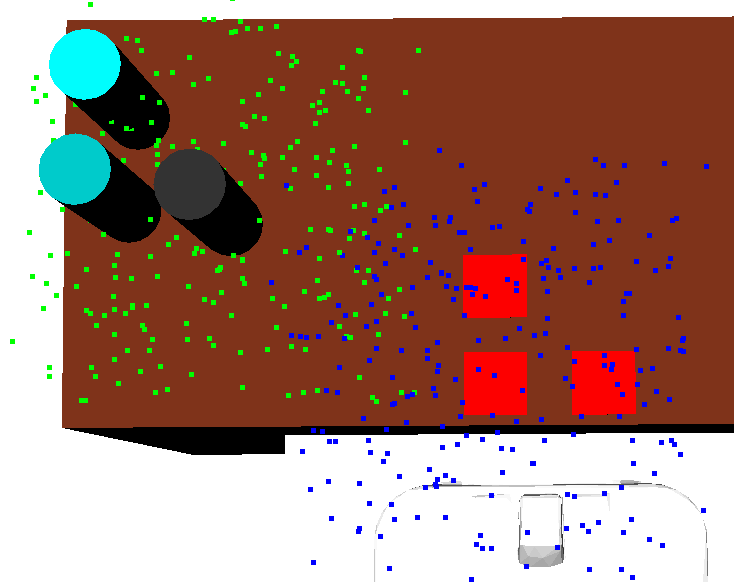
\includegraphics[width=\textwidth]{images/learns.png}
    \caption{Initial distribution}
  \end{subfigure}
  \begin{subfigure}[b]{0.4\linewidth}
    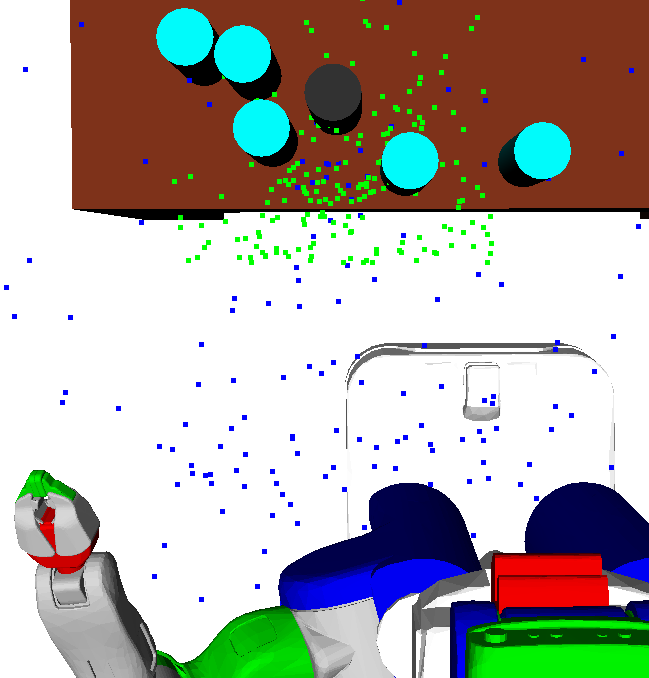
\includegraphics[width=\textwidth]{images/learn4.png}
    \caption{After 4 iterations.}
  \end{subfigure}
  \begin{subfigure}[b]{0.35\linewidth}
    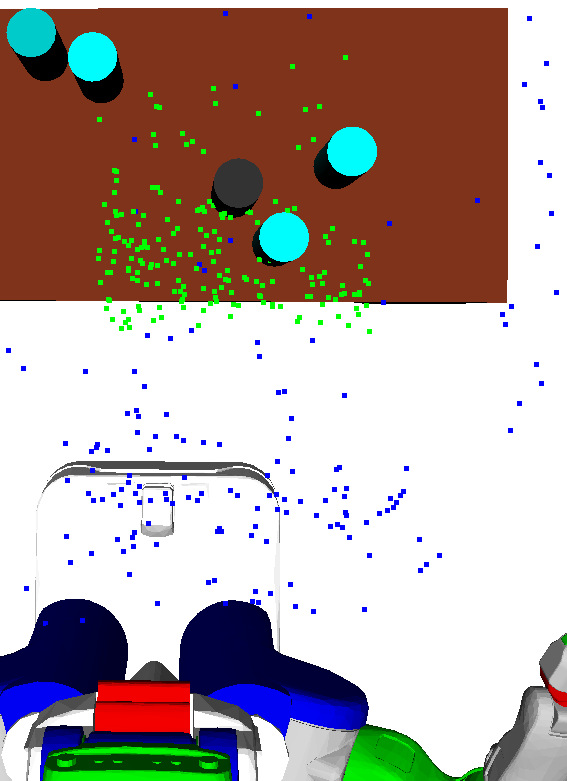
\includegraphics[width=\textwidth]{images/learn8.png}
    \caption{After 8 iterations.}
  \end{subfigure}
  \begin{subfigure}[b]{0.35\linewidth}
    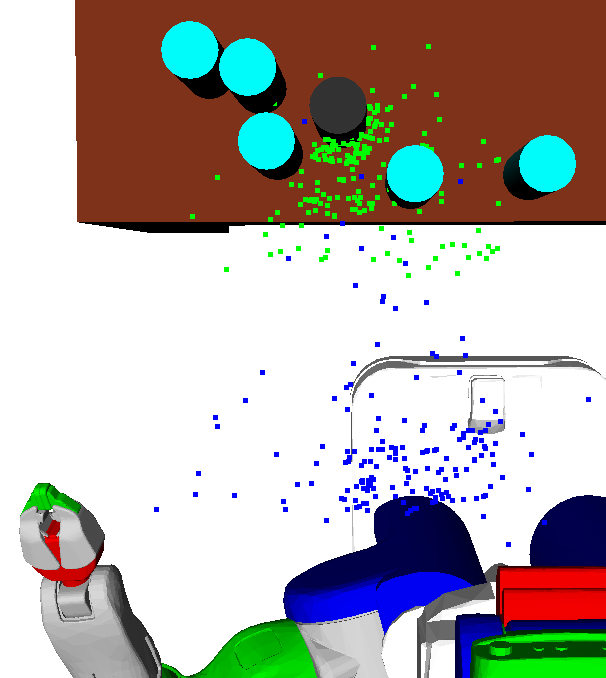
\includegraphics[width=\textwidth]{images/learn12.png}
    \caption{Final distribution.}
  \end{subfigure}
  \caption{\small{Learned base position (blue) and left arm grasp (green) distributions used to
pick up the black can after different training iterations for learning refinement policies.
An iteration refers to a single planning problem,
which terminates after $L$ calls to the \textsc{resample} routine. The
initial distributions are uniform because we initialize weights to $\vec{\mathbf{0}}$.
The final distributions are after 12 iterations.}}
  \label{fig:training}
  \vspace{-1.5 em}
\end{figure}

% \begin{figure}
%   \centering
%   \begin{subfigure}[b]{0.3\linewidth}
%     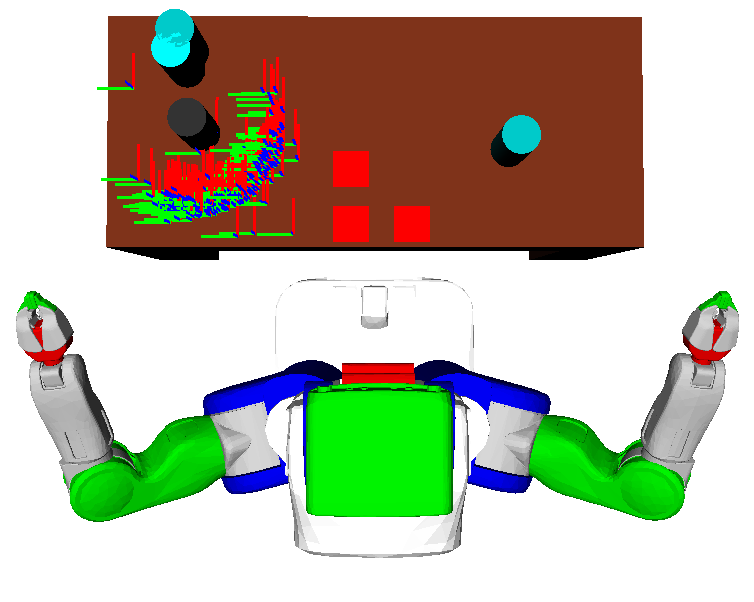
\includegraphics[width=\textwidth]{images/finalgraspnoobstr.png}
%     \caption{}
%   \end{subfigure}
%   \begin{subfigure}[b]{0.3\linewidth}
%     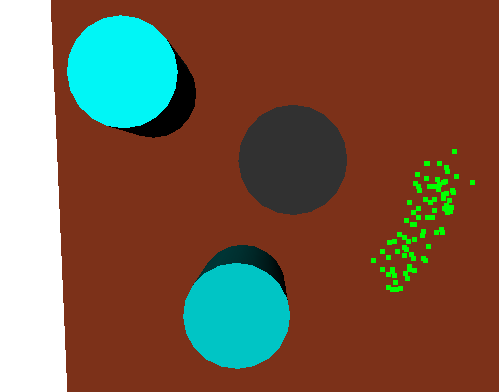
\includegraphics[width=\textwidth]{images/finalgraspobstr.png}
%     \caption{}
%   \end{subfigure}
%   \begin{subfigure}[b]{0.3\linewidth}
%     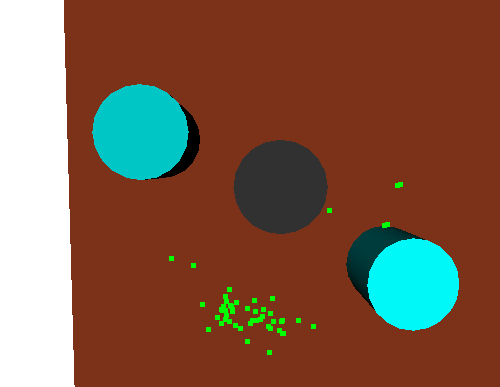
\includegraphics[width=\textwidth]{images/finalgraspobstr2.png}
%     \caption{}
%   \end{subfigure}
%   \caption{The learned grasp pose distribution
% is shown with different obstruction layouts. The system learns to
% avoid obstructions while providing a good set of grasping poses.}
%   \label{fig:obstr}
% \end{figure}

\begin{table}[t]
  \centering
  \vspace{8pt}
  \tabcolsep=0.11cm{
  \begin{tabular}{ccccc}
    \toprule[1.5pt]
      \textbf{\# Objects} & \textbf{System} & \textbf{\% Solved (SD)} & \textbf{Avg MP Time (s)} & \textbf{Avg \# MP Calls}\\
    \midrule[2pt]
      2 (dinner) & B & 100 (0) & 25.6 & 59.2\\
    \midrule
      2 (dinner) & L & 99 (2.0) & 26.0 & 61.6\\
    \midrule[1.5pt]
      4 (dinner) & B & 92 (0) & 45.8 & 94.5\\
    \midrule
      4 (dinner) & L & 99 (1.6) & 39.5 & 96.2\\
    \midrule[1.5pt]
      25 (cans) & B & 74 (0) & 15.1 & 19.0\\
    \midrule
      25 (cans) & L & 84 (5.1) & 12.4 & 12.6\\
    \midrule
      25 (cans) & F & 92 (5.8) & 10.7 & 12.0\\
    \midrule[1.5pt]
      30 (cans) & B & 36 (0) & 48.2 & 35.4\\
    \midrule
      30 (cans) & L & 69 (8.0) & 21.9 & 19.0\\
    \midrule
      30 (cans) & F & 77 (6.5) & 23.1 & 21.8\\
    \bottomrule[1.5pt]
  \end{tabular}}
  \caption{\small{Percent solved and standard deviation, along with time spent motion planning and number of calls to the motion
planner for the baseline system (B), our learned refinement policies with depth-first search through the plan refinement graph (L),
and our learned refinement policies and heuristics for searching the graph (F). Results for L and F
are averaged across 10 separately trained sets of weights. Time limit: 300s.}}
  \label{table:results}
  \vspace{-2 em}
\end{table}

\subsection{Training Methodology}
We use the reward function described earlier. Our weight
vectors are initialized to $\vec{\mathbf{0}}$ for all parameter types -- this
initialization represents a uniform distribution across the limits of the geometric search space.
We use 24 features for learning the $\theta_{p}$. 9 binary features encode the bucketed distance between the sample
and target (the object referenced by the parameter). 9 binary features encode the bucketed sample height. 3 features
describe the number of other objects within discs of radius 7, 10, and 15 centimeters around the
sample. 3 binary features describe the angle made between the vector from the
robot to the target and the vector from the sample to the target: whether the angle is less than
$\pi/3$, $\pi/2$, and $3\pi/4$.

Initial experimentation revealed that training weights for all parameter types jointly is intractable,
because planning takes a long time. Potential solutions for this would explore alternative RL algorithms,
but this is not our focus. Instead, we apply curriculum learning by training with a planning problem distribution
$\Prob$ that gets progressively harder. Additionally, we train the refinement policies first, then fix them while
training the graph search heuristics.

We evaluate our approach in two distinct domains: cans distributed on a table (the \emph{can domain})
and setting up bowls for dinner (the \emph{dinner domain}).
We compare performance with a baseline that uses the hand-coded sampling distributions
in Srivastava et al.~\cite{srivastava2014combined} and depth-first search of the
plan refinement graph, which always refines the plan that incorporates all error information obtained
thus far. For the can domain, we report results for 3 systems: 1) this baseline, 2) our learned refinement policies
with the depth-first search, and 3) our learned refinement policies and graph search heuristics.
For the dinner domain, we report results only for the first 2 systems, because the errors propagated in this
domain relate to the stackability of objects. Since this is independent of continuous parameter instantiations, we want to
incorporate all available error information when attempting refinement. Thus, depth-first search can be expected to perform well
in this setting.

For the third system, which trains a refinement policy and graph search heuristics, we employ the following
algorithm to produce a trained set of weights. We train 3 sets independently, test each
one on a validation set of 50 environments, and output the best-performing one. We found that this
reduced variation due to random seeding. For the second system, by contrast, we train a single
set of weights and output it, without any validation.

We report results on a fixed test set of 50 randomly generated environments.
For the second and third systems, we average across running the training process 10 times
and evaluating each final set of weights separately.

Our experiments are conducted in Python 2.7 using the OpenRave simulator~\cite{Diankov_2008_6117} with a PR2 robot.
The motion planner we use is trajopt~\cite{schulman2013finding}, and the task planner is Fast-Forward~\cite{FF}.
The experiments were carried out in series on an Intel Core i7-4790K machine with 16GB RAM.
Table \ref{table:results} summarizes our quantitative results, and \figref{fig:cover} and \figref{fig:training}
show learned refinement policies.

\subsection{Can Domain}
We run two sets of experiments, using 25 objects and 30 objects on the table.
The goal across all experiments is for the robot to pick up a particular object with its
left gripper. We disabled the right gripper, so any obstructions to the target object must be picked up and
placed elsewhere on the table. This domain has 4 types of continuous parameters: base poses, object grasp
poses, object putdown poses, and object putdown locations onto the table.
% The range of allowable values for grasp and putdown poses is a cube of side length 30 centimeters around the
% target object or putdown location. For base poses, the range is a square of side length 1 meter around the
% object or location which the robot is approaching. For putdown locations, the range is defined by the table.

Our curriculum learning system first trains base poses and grasp poses for $N = 12$ iterations with $\epsilon = 5$,
then base poses, grasp poses, and putdown poses (at fixed location) for $N = 18$ iterations with $\epsilon = 20$,
then all parameter types for $N = 30$ iterations with $\epsilon = 20$. We fixed $L = 100$.

The results demonstrate significant improvements in performance to the baseline system for success rate, motion planning
time, and number of motion planner calls. For the 30 object case, though,
there is an increase in average motion planning time when we use trained graph search heuristics. This is likely because of suboptimal
search decisions occasionally being made.

\subsection{Dinner Domain}
We run two sets of experiments, using 2 and 4 bowls. The robot must move the
bowls from their initial locations on one table to target locations on the other. We assign a cost to
base motion in the environment, so the robot is encouraged to use the provided tray, onto which bowls can be stacked.
This domain has 5 types of continuous parameters: base poses, object grasp poses, object putdown poses, tray pickup
poses, and tray putdown poses.

Our curriculum learning system first trains base poses and tray pickup and putdown poses for
$N = 20$ iterations, then object grasp and putdown poses for $N = 20$ iterations. We fixed $L = 100$ and $\epsilon = 10$.

The results demonstrate comparable performance to the baseline system. The reason is that
hand-coded discretizations of the sample space are very good in this domain. For example, the optimal
robot base pose from which to pick up the tray is directly in front of it, which is quickly sampled through
the baseline system's discretization.